%%%%%%%%%%%%%%%%%%%%%%%%%%%%%%%%%%%%%%%%%
% Stylish Article
% LaTeX Template
% Version 2.1 (1/10/15)
%
% This template has been downloaded from:
% http://www.LaTeXTemplates.com
%
% Original author:
% Mathias Legrand (legrand.mathias@gmail.com) 
% With extensive modifications by:
% Vel (vel@latextemplates.com)
%
% License:
% CC BY-NC-SA 3.0 (http://creativecommons.org/licenses/by-nc-sa/3.0/)
%
%%%%%%%%%%%%%%%%%%%%%%%%%%%%%%%%%%%%%%%%%

%----------------------------------------------------------------------------------------
%	PACKAGES AND OTHER DOCUMENT CONFIGURATIONS
%----------------------------------------------------------------------------------------

\documentclass[fleqn,10pt]{SelfArx}
\usepackage[backend=biber]{biblatex}
\addbibresource{references.bib}
\usepackage[english]{babel}
\usepackage{graphicx}
\graphicspath{ {./imgs/} }


%----------------------------------------------------------------------------------------
%	COLUMNS
%----------------------------------------------------------------------------------------

\setlength{\columnsep}{0.55cm} % Distance between the two columns
\setlength{\fboxrule}{0.5pt} % Width of the border around the abstract

%----------------------------------------------------------------------------------------
%	COLORS
%----------------------------------------------------------------------------------------

\definecolor{color1}{RGB}{0,0,90} % Color of the article title and sections
\definecolor{color2}{RGB}{0,20,20} % Color of the boxes behind the abstract and headings

%----------------------------------------------------------------------------------------
%	HYPERLINKS
%----------------------------------------------------------------------------------------

\usepackage{hyperref} % Required for hyperlinks
\hypersetup{hidelinks,colorlinks,breaklinks=true,urlcolor=color2,citecolor=color1,linkcolor=color1,bookmarksopen=false,pdftitle={Title},pdfauthor={Author}}

%----------------------------------------------------------------------------------------
%	ARTICLE INFORMATION
%----------------------------------------------------------------------------------------

\JournalInfo{Università degli Studi di Milano Bicocca - DISCO}
\Archive{a.a. 2019/20}

\PaperTitle{Amazon Kindle Store Reviews}

\Authors{
  Federico Moiraghi [799735] -
  Pranav Kasela [846965] -
  Roberto Berlucchi [847939]
}

\Keywords{}
\newcommand{\keywordname}{Keywords}

%----------------------------------------------------------------------------------------
%	ABSTRACT
%----------------------------------------------------------------------------------------

\Abstract{ % TODO: abstract is written at the end of the whole report
  The present Project is composed by two parts: in the first part it is provided a model to predict if the buyer of a e-book on Amazon's Kindle Store liked it or not according to the text of the comment; in the second part...
}

%----------------------------------------------------------------------------------------

\begin{document}

\flushbottom % Makes all text pages the same height

\maketitle
\tableofcontents
\newpage

\thispagestyle{empty} % Removes page numbering from the first page

%----------------------------------------------------------------------------------------
%	ARTICLE CONTENTS
%----------------------------------------------------------------------------------------

\section*{Introduction}
\addcontentsline{toc}{section}{Introduction}

The present Project is divided into several parts, starting from the same corpus (Amazon's Kindle Store reviews\footnote{\url{https://nijianmo.github.io/amazon/index.html}}), with different purposes.
In the first part, the aim is to provide a good supervised model to predict if a user liked the book or not according to his or her review.\newline
% TODO: add descriptions of other parts
\newline

The entire Project\footnote{Original code is available on GitHub at the link \url{https://github.com/moiraghif/Amazon-Rating-Prediction}} is made using Apache Hadoop\footnote{\url{https://hadoop.apache.org/}} (for data pre-processing) and Apache Spark\footnote{https://spark.apache.org/} (for the analysis) and is distributed as Dock image through DockHub\footnote{\url{pkasela/amazon_review_hadoop_spark}}.
Using a Big Data framework is required by the huge quantity of texts, hardly analyzable by a single machine without taking some precautions: this Project aims not only to provide a valid approach to all tasks but also to propose a scalable and efficient way to solve them.
Distribution through Docker is considered necessary to simplify installation of dependencies: providing a virtual Operating System (in the specific case, Linux Ubuntu 16.04) with all programs already installed and configured is useful to focus the attention on the \textit{Natural Language Processing} (NLP) pipeline instead of building the environment.

It is chosen Kindle Store corpus to avoid problems that physical products reviews have in common: a lot of reviews do not focus on the product itself but stress how it was delivered.
Another reason to limit the analysis to the Kindle Store corpus is the fact that its size on disk does not require a cluster (the entire Amazon corpus weights about \verb|700Gb|) but can be processed by a single machine in a reasonable time.

% ------------------------------------------------

\newpage
\section{Preprocessing and Data Cleaning}
As the dataset is composed by real reviews from Amazon's Kindle Store, the cleaning part is fundamental to reach good performance on all tasks.
The file is in \verb|.json| format and contains approximately $5 \cdot 10^6$ observations ($5,722,988$ reviews of $493,859$ products) coming from Amazon U.S.A. Kindle Store in a period starting from May 1996 to October 2018.
For each observation some recordings are reported, such as ID of the product, of the reviewer, timestamp (in seconds from epoch), text, rating (number of stars from 1 up to 5) and votes of the review (given by other users).
Fields of interest are selected using a series of regular expression (regex) to parse the \verb|.json| string, instead of the official Python's \verb|json| library, obtaining a $20\%$ gain in speed. \newline

Reviews are written for the most in English, but a small fraction (approximately $5\%$) is composed by texts written in other languages (for the most Spanish or French) or contains just emoticons.
For the purpose of this Project, those reviews are just ignored to avoid the additional complexity caused by the multilingual case.
\verb|CLD-2|\cite{cld2} library is used to filter reviews by language, removing those that are not in English or do not contain text: it uses a Recurrent Neural Network (RNN) to implement a character-level analysis of the text and predict its language.
This library is selected among others due to its high speed in managing the quantity of data used in the Project: a comparison made by authors shows that it is more than 200 times faster than Google's \verb|langdetect| and achieves comparable performances\cite[6]{cld2}: \newline
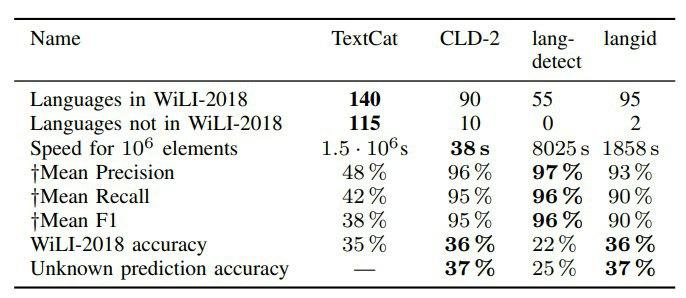
\includegraphics[width=\linewidth]{languages}
\newline
After this first phase of cleaning, data is stored in a structured form on the Hadoop file-system (HDFS) and is parsed by a series of regular expression to make it more clean:
\begin{itemize}[noitemsep]
\item HTML tags and URLs are removed;
\item punctuation is normalized (e.g. four or more consecutive points are reduced to three);
\item contractions are re-written in extended form;
\item particular constructions are re-written in simplified form (e.g. ``have to'' $\rightarrow$ ``must'', ``is going to'' $\rightarrow$ ``will'');
\item domain-specific terms are simplified (e.g. ``ebook'' $\rightarrow$ ``book'', all Amazon's offers becomes ``Amazon'', all Kindle e-book readers becomes ``kindle'');
\item numbers are re-written according to their semantics (when easily understandable by the context) or removed (e.g. all prices becomes ``money'');
\item modal verbs are lemmatized;
\item words with emphatic repetition of a letter are normalized;
\item remaining contractions or words composed by a single letter are removed;
\item punctuation is removed.
\end{itemize}
After this pipeline, the text is processed by a SpaCy\footnote{\url{https://spacy.io/}} model that tokenize sentences and words within each sentence (using a \textit{Deep Learning} approach); each word is then either stemmatized by Porter's Stemmer (second version) offered by NLTK\footnote{\url{http://www.nltk.org/}} or removed if it is a \textit{stopwords}.
Stopwords are taken from NLTK's English list, from which negations and some prepositions are removed, and with the addition of some domain-specific words (such as ``book'' or ``author''). \newline

The entire process, composed by two \textit{only-mapping} jobs, takes less than one hour on a single machine, due to high efficiency provided by HDFS' parallel distribution of the work.
After this process, data is rewritten on the HDFS in a more clean format and is ready to be analyzed.

\newpage
\section{Task 1: Classification}
The first task is to predict if a user liked the book or not according only on the text of the review (a binary-classification task).
Target variable is a binary transformation of the number of stars of the review: if the user gave four of five stars to the book, it is considered ``liked''; on the other hand, if the user gave three or less stars, he or she does ``not like'' the book.

\subsection{Exploratory Analysis}
Original ratings given by users are not distributed equally: following table shows that more than $80\%$ of reviews give four or five stars to the ebook.
\begin{center}
  \begin{tabular}{l|r}
    stars & frequency \\
    \hline
    1 star  & $257,185$ \\
    2 stars & $212,912$ \\
    3 stars & $477,640$ \\
    4 stars & $1,202,145$ \\
    5 stars & $3,323,996$
  \end{tabular}
\end{center}
But, having $5,473,878$ observations, this percentage is not considered problematic.
In fact, Apache Spark, in the case of binary classification, does not compute \textit{accuracy} but \textit{AUC} (\textit{Area Under - ROC - Curve}), that is much more informative for unbalanced classes: after a simple optimization pipeline, the resulting model should not be influenced by the unbalance of classes.

\subsection{Classification Pipeline}
Loading the cleaned text from HDFS, all analysis is made directly in Spark with a simple pipeline that uses a 3-folds cross validation to estimate performance (using the mean) in a grid search:
\begin{itemize}[noitemsep]
\item target variable is binarized;
\item text is tokenized with a simple regex-tokenizer;
\item $n$-grams are extracted;
\item \textit{Tf-Idf} matrix is calculated (\textit{Idf} values are trained only on the \textit{train set}), removing columns with less than 5 occurrences (considered \textit{noise} according to Zipf's Law);
\item \textit{Tf-Idf} values are used to train a logistic model (using only the \textit{train set});
\item $AUC$ is computed on the \textit{test set}.
\end{itemize}
Parameters of search for the grid-search optimization are the size of $n$-grams (starting from 1 up to 3) and the learning rate of the logistic regression (that is computed iteratively for optimization).

\subsection{Results and Interpretation}
Results of the optimization process are the following (on rows $n$-grams size, on columns \textit{learning rate} value):
\begin{center}
  \begin{tabular}[center]{l|c c c}
      & 0.1 & 0.05 & 0.01 \\
    \hline
    1 & 0.90306 & 0.90317 & 0.90141 \\
    2 & 0.90640 & 0.90395 & 0.89798 \\
    3 & 0.77204 & 0.76828 & 0.76119
  \end{tabular}
\end{center}
As the table shows, the best configuration found in the process is using \textit{bi-grams} with a high \textit{learning rate}.
Poor performances yielded by the use of \textit{three-grams} can be justified by an insufficient quantity of data: resulting matrix is very high-dimensional, so the risk of \textit{overfitting} the \textit{train set} is very high.
On the other hand, while using \textit{bi-grams} produces a matrix bigger than one obtained by \textit{mono-grams}, it catches some constructions with semantics (such as name and surname of the author): for this reason their use performs better.
\textit{Three-grams} on the other hand catch even more complex constructions, but lack of data make them unusable.

\subsection{Possible Improvements}
Due to higher performance of \textit{bi-grams} instead of \textit{mono-grams}, one strategy to improve results consists of using a simple Ontology to support the tokenization of texts, replacing names of authors, characters or titles with the corresponding URI; in alternative, an Entity Recognition algorithm can be used.
This is a very aggressive way to normalize names and titles, so that constructions such as ``name + surname'' are represented by just one token.

\subsection{Possible Uses of the Model}
Using texts written in natural language in a informal context, the Model should generalize well on texts taken from other social media (such as Facebook or Twitter).
This model therefore can be tested on social media platforms to make market research or to integrate data from different sources in a Recommending System.

\newpage
\section{Task 2: Clustering}
TODO
%----------------------------------------------------------------------------------------
%	REFERENCE LIST
% ----------------------------------------------------------------------------------------
\newpage
\hfill
\newpage
\section{Conculsions}
TODO
\newpage
\printbibliography


%----------------------------------------------------------------------------------------

\end{document}